Si è quindi proceduto all’addestramento della rete tramite Python usando TensorFlow e le API di Keras. Si è reso necessario modificare il file \textit{pipeline.config} adattandolo alle nostre esigenze:

\begin{itemize}
    \item \textit{numclasses} che corrisponde al numero di item da identificare;
    \item \textit{path} vari da adattare al nostro workspace, tra cui il path per i checkpoint, per i record di input e per il labelmap.
\end{itemize}

Durante il procedimento di training si sono tenuti controllati i valori della nostra rete. In particolare, abbiamo usato \textbf{Tensorboard}: un framework grafico utile a capire l'andamento della nostra rete, infatti abbiamo avuto modo di controllare ad ogni training le performance della nostra rete di machine learning.

TensorBoard fornisce la visualizzazione e gli strumenti necessari per la sperimentazione del machine learning:

\begin{itemize}
    \item Monitoraggio e visualizzazione di metriche come perdita e precisione;
    \item Visualizzazione del grafico del modello (operazioni e livelli);
    \item Visualizzazione degli istogrammi di pesi, distorsioni o altri tensori man mano che cambiano nel tempo.
\end{itemize}

\begin{figure}[htbp]
    \centering
    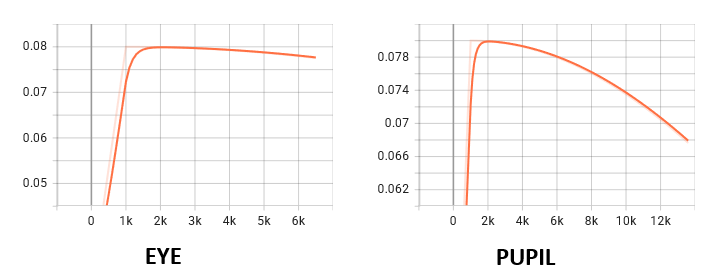
\includegraphics[scale=0.7]{ReteNeurale/EyeDetection/Training/Images/learning_rate_both_edited.png}
    \caption{Tensorboard Learning\_rate}
    \label{fig:eyelearningrate}
\end{figure}

Si è ottenuto in output un modello addestrato e pronto all’uso.

\begin{figure}[htbp]
    \centering
    \subfigure[Test personaggio famoso]{
    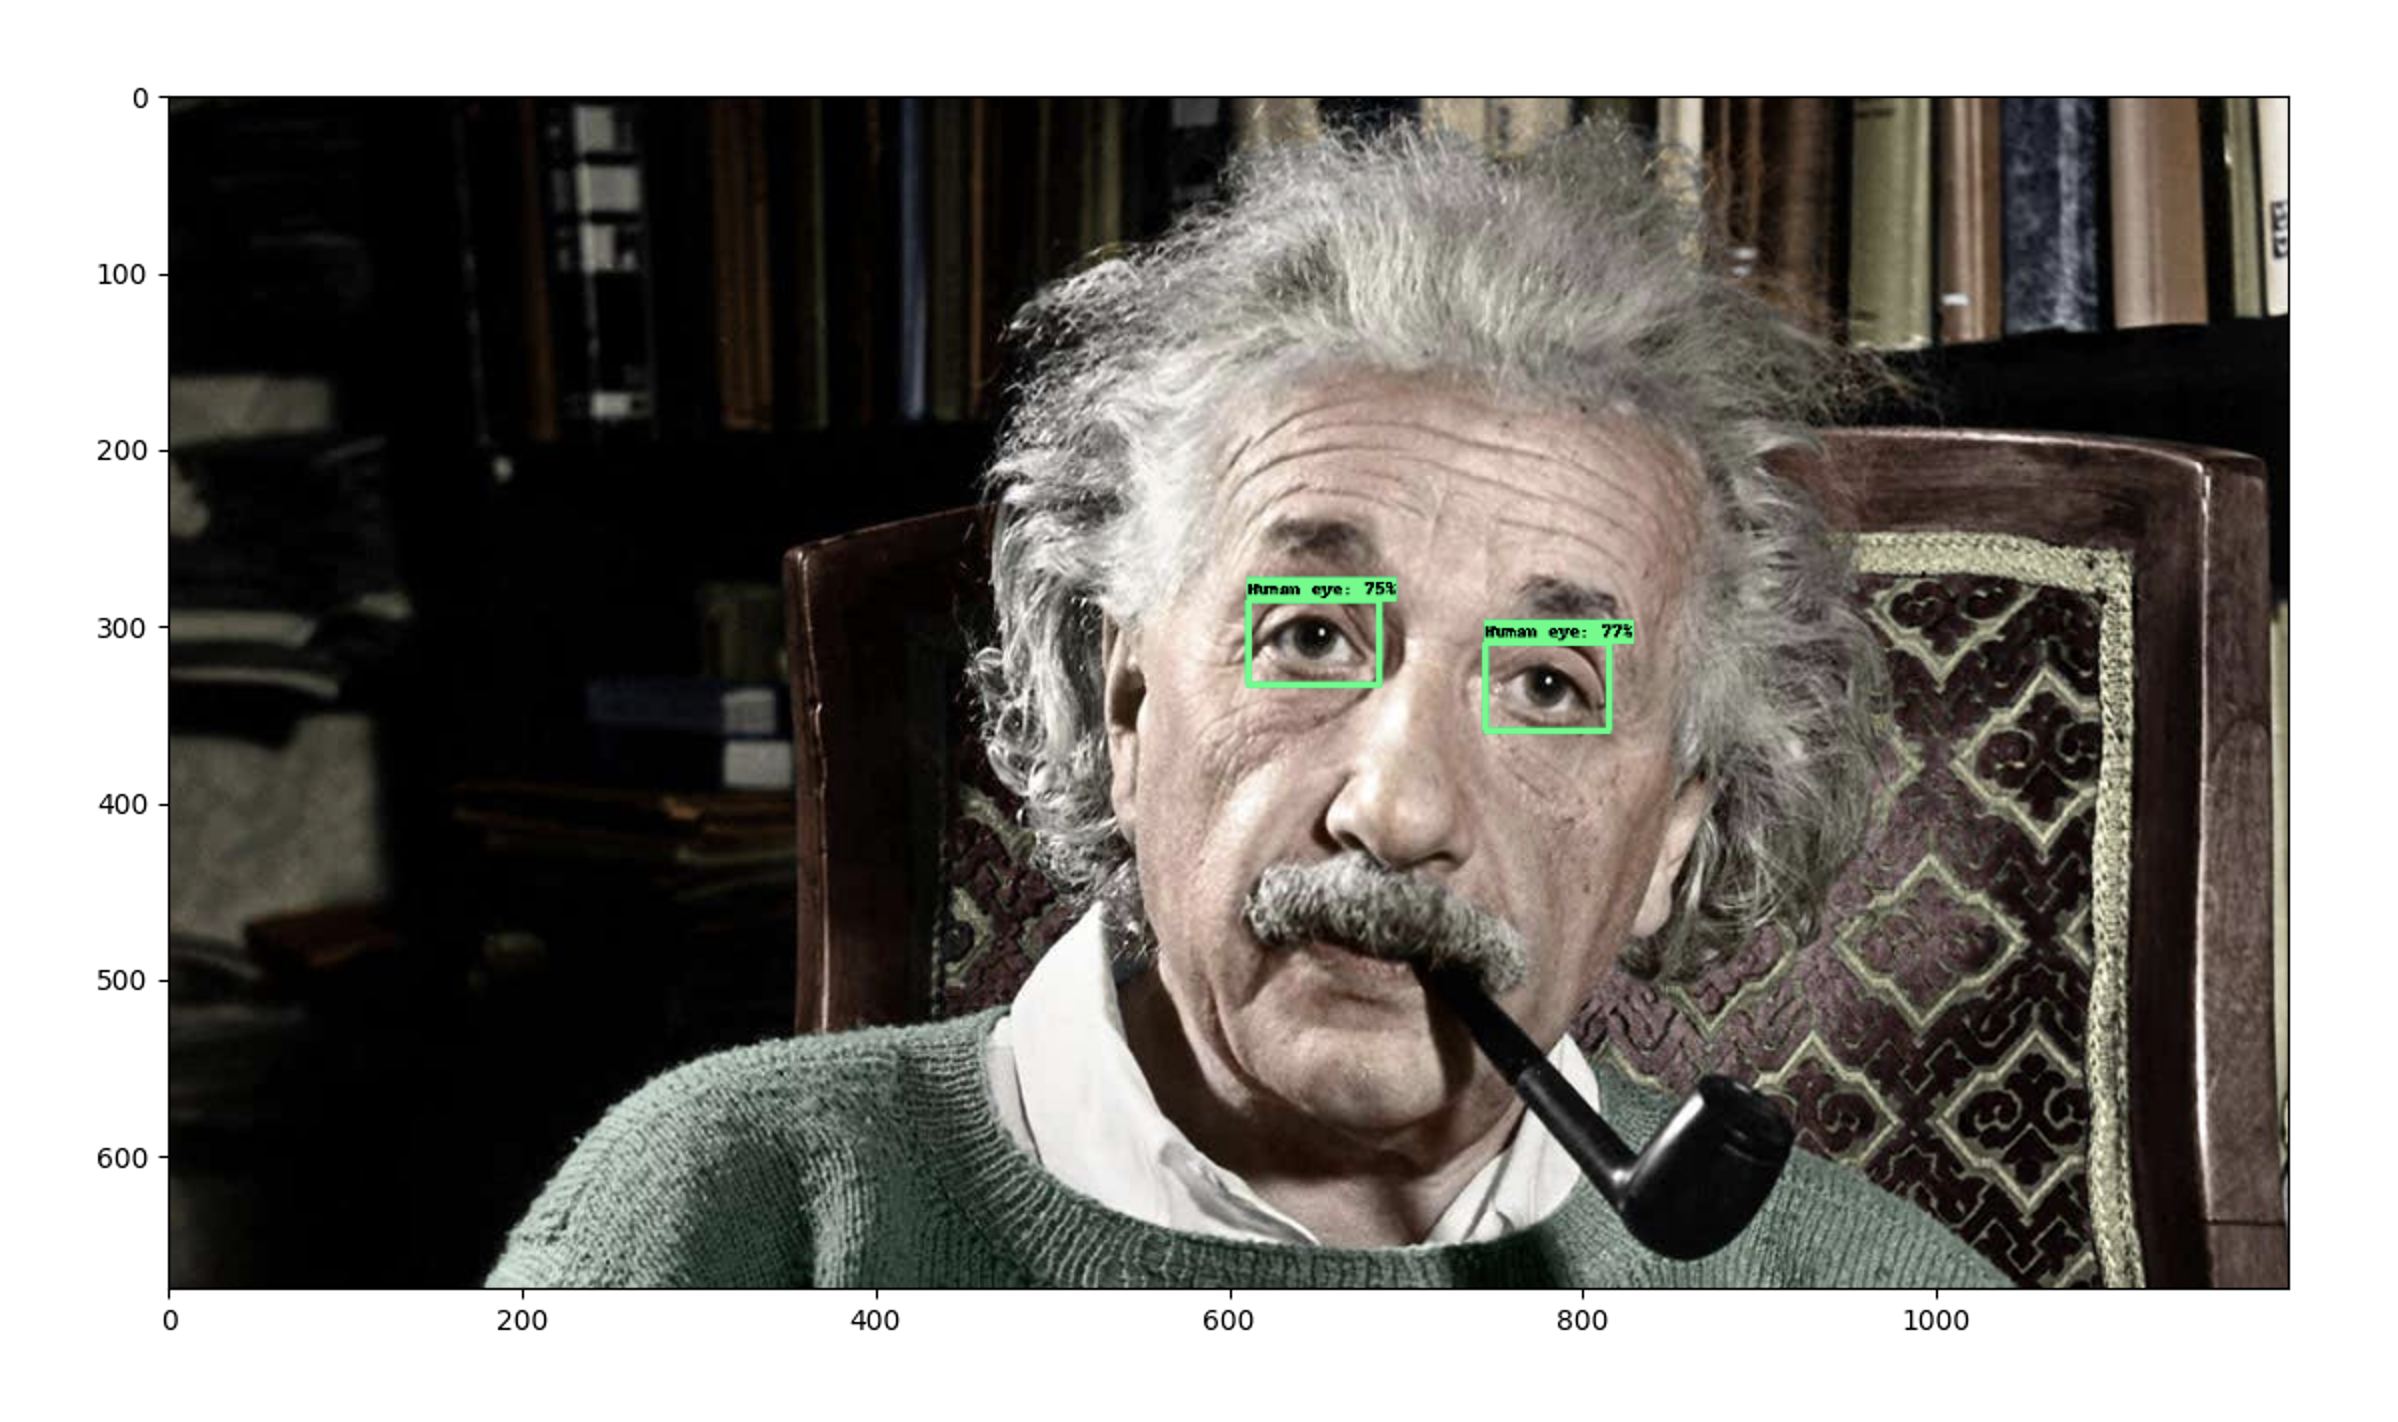
\includegraphics[scale=0.16]{ReteNeurale/EyeDetection/Training/Images/einstein.png}
    \label{fig:testeyeinstein}
    }
    \hspace{5mm}
    \subfigure[Test multiplo]{
    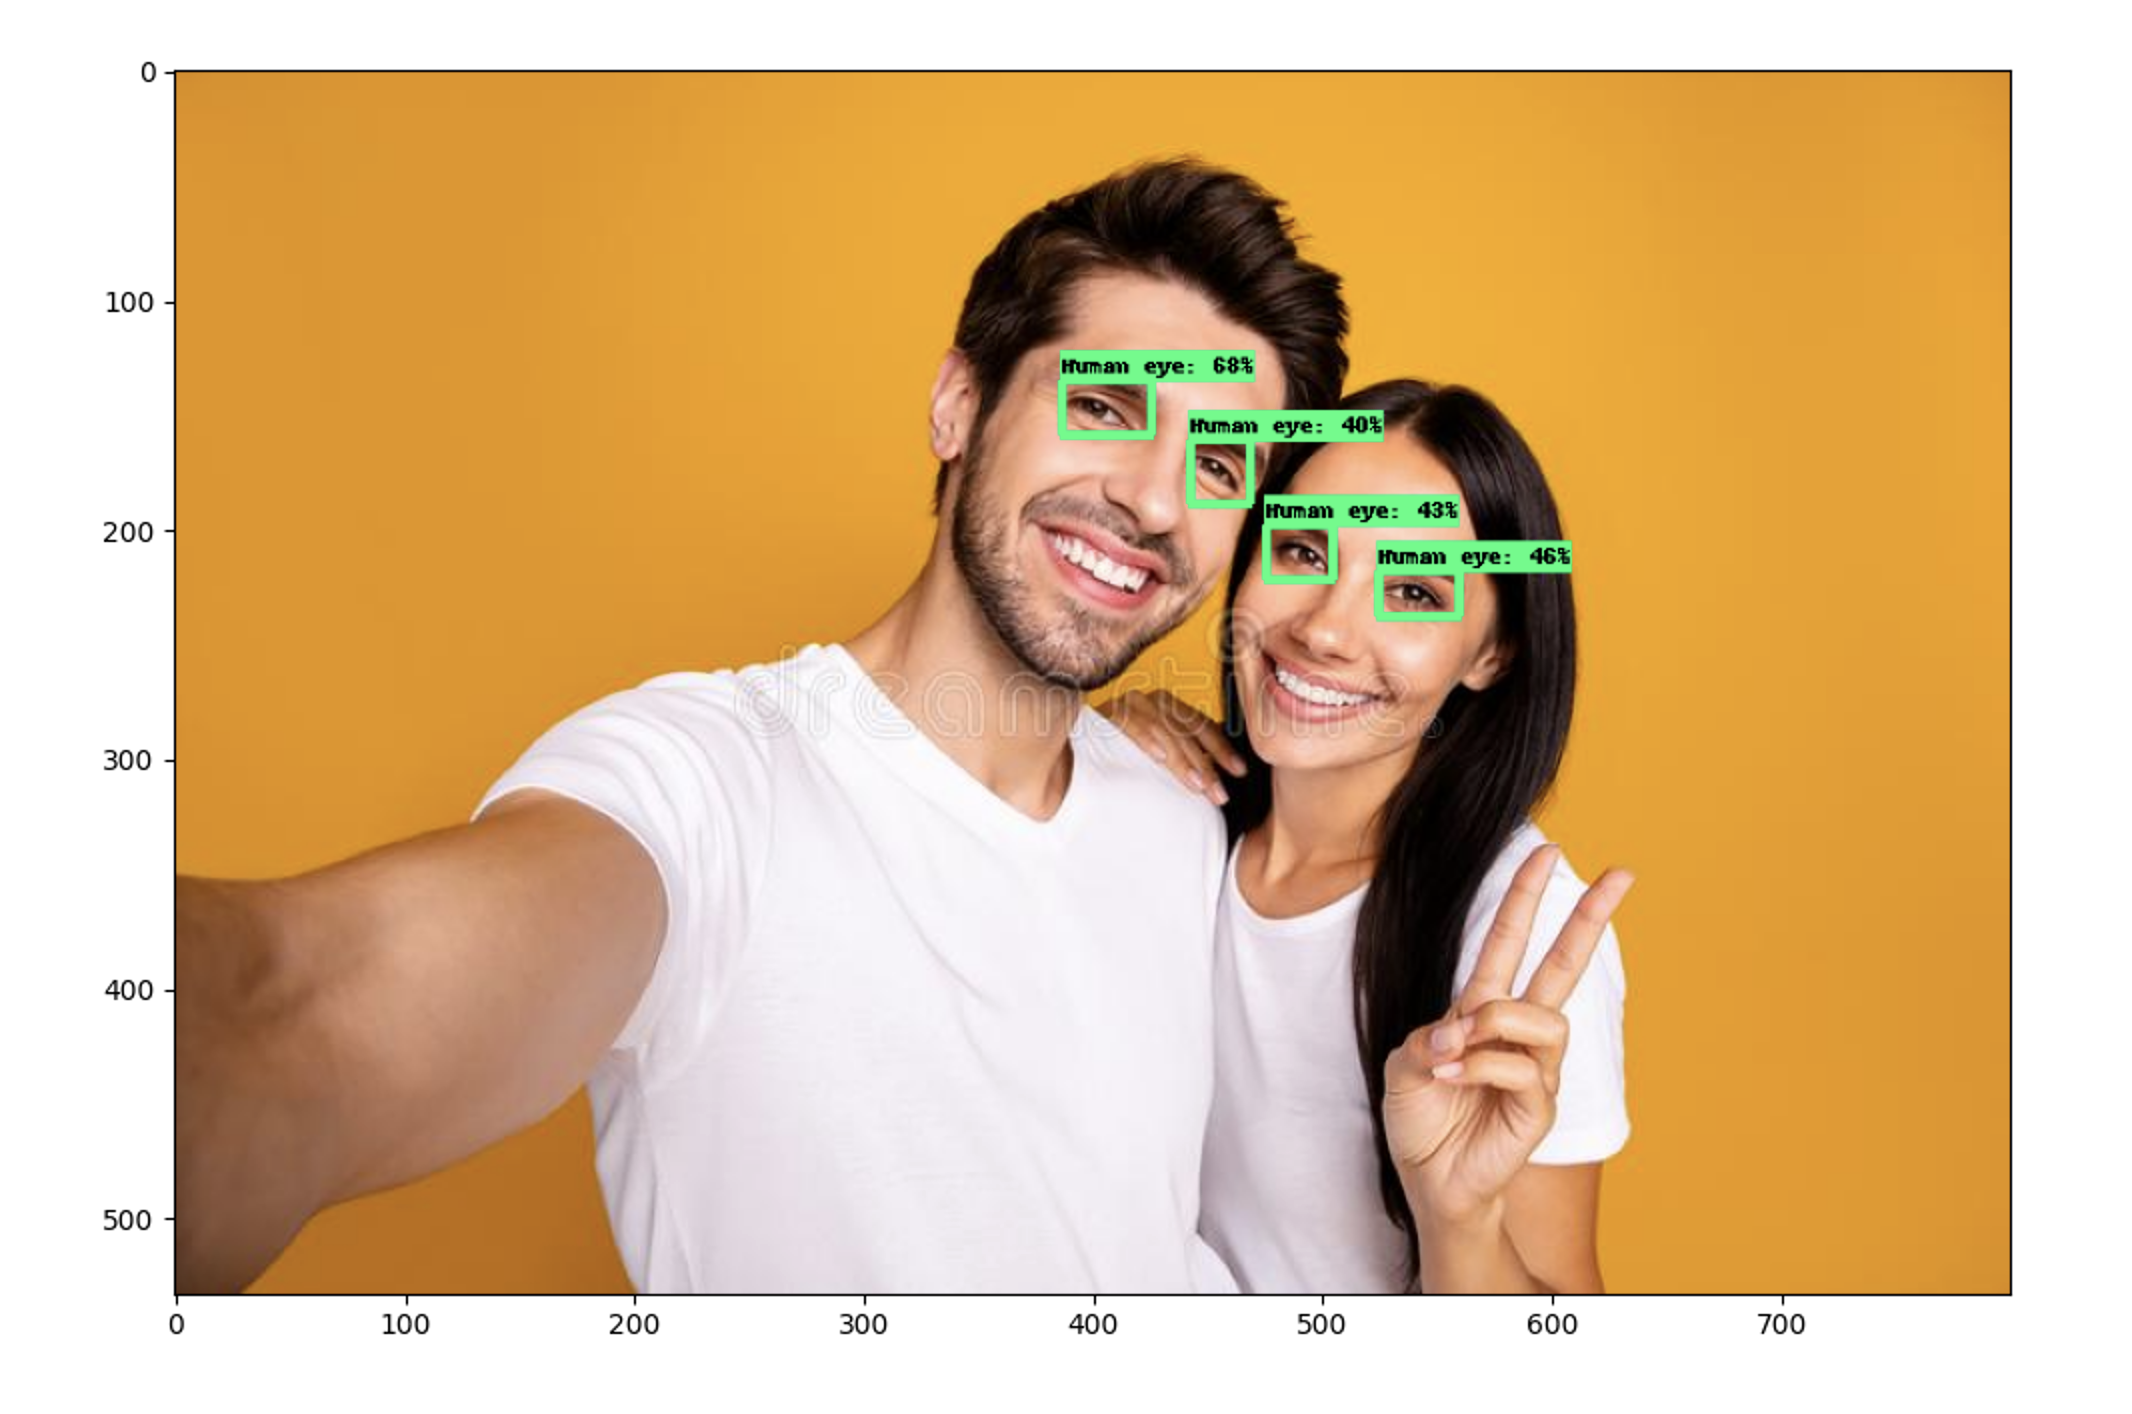
\includegraphics[scale=0.16]{ReteNeurale/EyeDetection/Training/Images/gruppo.png}
    \label{fig:testeyegruppo}
    }
    \caption{Test Eye-Tracking}
    \label{fig:testeyetracking}
\end{figure}

Prima di testare direttamente su Android, abbiamo deciso prima di testare e analizzare la nostra nuova rete utilizzando la libreria Matplotlib, utile per visualizzare graficamente via shell i nostri risultati. In particolare abbiamo usato \textbf{Tkinter}, l'unico framework GUI incluso nella libreria standard di Python.

A fini di testing si è preso ad esempio il volto di un
personaggio pubblico, quello di Albert Einstein, e anche un'immagine contenente più persone in modo tale da poter verificare la correttezza e la precisione della rete anche in condizioni più difficili.